\documentclass{standalone}
\usepackage{tikz}
\usetikzlibrary{patterns}
\usetikzlibrary{positioning}
\usetikzlibrary{patterns, positioning}
\usetikzlibrary{shapes.misc}
\usepackage[outline]{contour}
\contourlength{1.5pt} 
\usepackage[sfdefault]{ClearSans}

\begin{document}
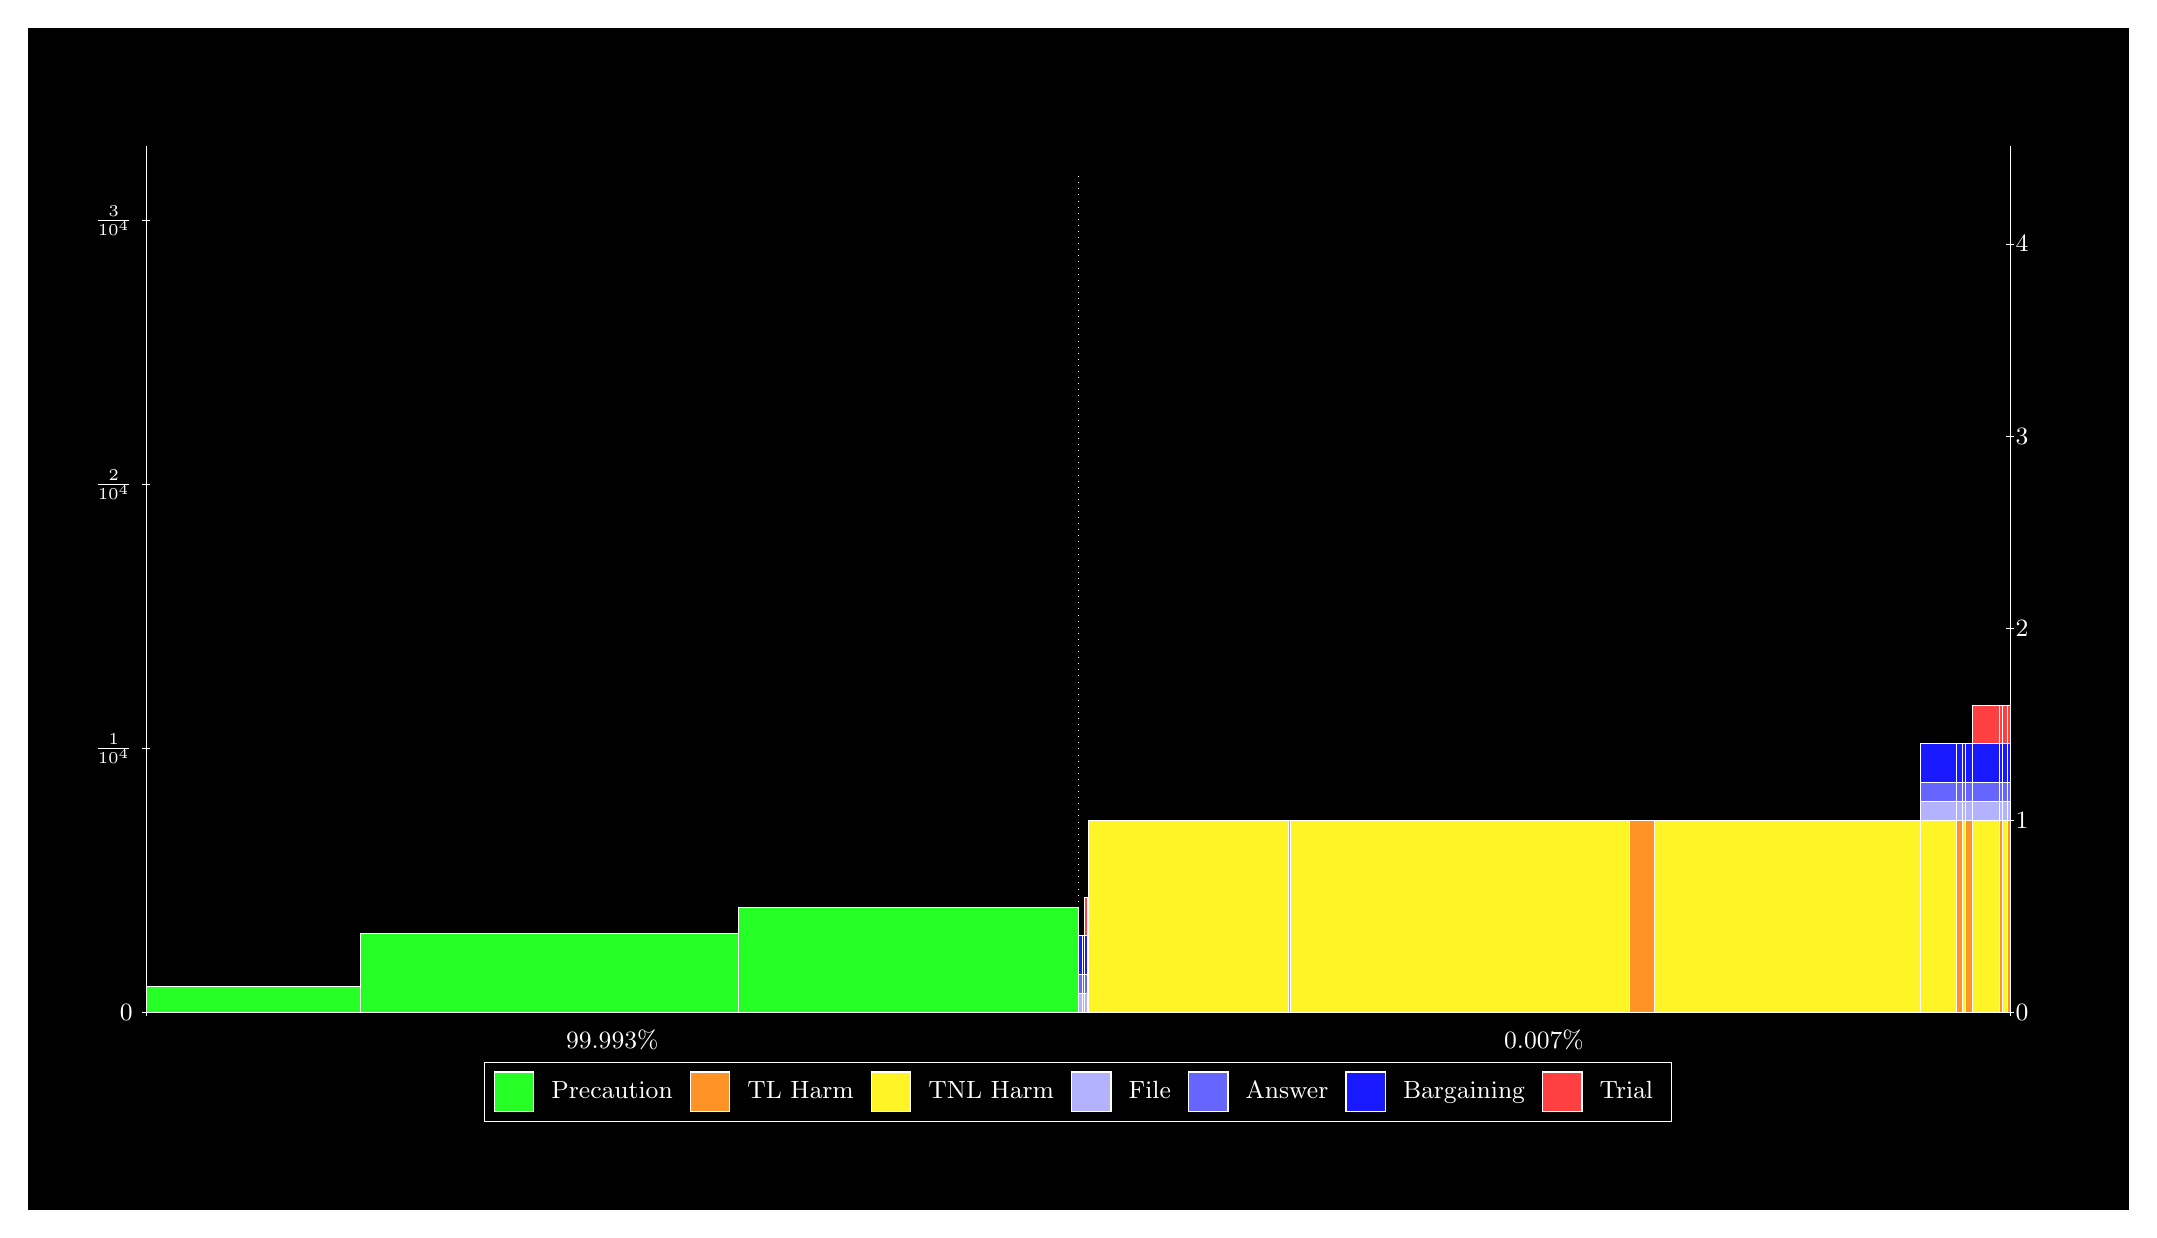
\begin{tikzpicture}
\draw[fill=black] (0,0) rectangle (26.667,15);
\draw[fill=green!85,draw=white,very thin] (1.5,2.5) rectangle (4.2218,2.8352);
\draw[fill=green!85,draw=white,very thin] (4.2218,2.5) rectangle (9.0126,3.5057);
\draw[fill=green!85,draw=white,very thin] (9.0126,2.5) rectangle (13.333,3.841);
\draw[fill=green!85,draw=white,very thin] (13.333,2.5) rectangle (13.391,2.5);
\draw[fill=blue!30,draw=white,very thin] (13.333,2.5) rectangle (13.391,2.744);
\draw[fill=blue!60,draw=white,very thin] (13.333,2.744) rectangle (13.391,2.9881);
\draw[fill=blue!90,draw=white,very thin] (13.333,2.9881) rectangle (13.391,3.4761);
\draw[fill=green!85,draw=white,very thin] (13.391,2.5) rectangle (13.412,2.5001);
\draw[fill=blue!30,draw=white,very thin] (13.391,2.5001) rectangle (13.412,2.7441);
\draw[fill=blue!60,draw=white,very thin] (13.391,2.7441) rectangle (13.412,2.9881);
\draw[fill=blue!90,draw=white,very thin] (13.391,2.9881) rectangle (13.412,3.4761);
\draw[fill=green!85,draw=white,very thin] (13.412,2.5) rectangle (13.453,2.5);
\draw[fill=blue!30,draw=white,very thin] (13.412,2.5) rectangle (13.453,2.744);
\draw[fill=blue!60,draw=white,very thin] (13.412,2.744) rectangle (13.453,2.9881);
\draw[fill=blue!90,draw=white,very thin] (13.412,2.9881) rectangle (13.453,3.4761);
\draw[fill=red!75,draw=white,very thin] (13.412,3.4761) rectangle (13.453,3.9641);
\draw[fill=green!85,draw=white,very thin] (13.453,2.5) rectangle (13.467,2.5001);
\draw[fill=blue!30,draw=white,very thin] (13.453,2.5001) rectangle (13.467,2.7441);
\draw[fill=blue!60,draw=white,very thin] (13.453,2.7441) rectangle (13.467,2.9881);
\draw[fill=blue!90,draw=white,very thin] (13.453,2.9881) rectangle (13.467,3.4761);
\draw[fill=red!75,draw=white,very thin] (13.453,3.4761) rectangle (13.467,3.9642);
\draw[fill=green!85,draw=white,very thin] (13.467,2.5) rectangle (16.008,2.5);
\draw[fill=yellow!85,draw=white,very thin] (13.467,2.5) rectangle (16.008,4.9402);
\draw[fill=green!85,draw=white,very thin] (16.008,2.5) rectangle (16.023,2.5);
\draw[fill=orange!85,draw=white,very thin] (16.008,2.5) rectangle (16.023,4.9402);
\draw[fill=green!85,draw=white,very thin] (16.023,2.5) rectangle (20.338,2.5001);
\draw[fill=yellow!85,draw=white,very thin] (16.023,2.5001) rectangle (20.338,4.9402);
\draw[fill=green!85,draw=white,very thin] (20.338,2.5) rectangle (20.65,2.5001);
\draw[fill=orange!85,draw=white,very thin] (20.338,2.5001) rectangle (20.65,4.9402);
\draw[fill=green!85,draw=white,very thin] (20.65,2.5) rectangle (24.033,2.5001);
\draw[fill=yellow!85,draw=white,very thin] (20.65,2.5001) rectangle (24.033,4.9403);
\draw[fill=green!85,draw=white,very thin] (24.033,2.5) rectangle (24.49,2.5);
\draw[fill=yellow!85,draw=white,very thin] (24.033,2.5) rectangle (24.49,4.9402);
\draw[fill=blue!30,draw=white,very thin] (24.033,4.9402) rectangle (24.49,5.1842);
\draw[fill=blue!60,draw=white,very thin] (24.033,5.1842) rectangle (24.49,5.4282);
\draw[fill=blue!90,draw=white,very thin] (24.033,5.4282) rectangle (24.49,5.9163);
\draw[fill=green!85,draw=white,very thin] (24.49,2.5) rectangle (24.556,2.5);
\draw[fill=orange!85,draw=white,very thin] (24.49,2.5) rectangle (24.556,4.9402);
\draw[fill=blue!30,draw=white,very thin] (24.49,4.9402) rectangle (24.556,5.1842);
\draw[fill=blue!60,draw=white,very thin] (24.49,5.1842) rectangle (24.556,5.4282);
\draw[fill=blue!90,draw=white,very thin] (24.49,5.4282) rectangle (24.556,5.9163);
\draw[fill=green!85,draw=white,very thin] (24.556,2.5) rectangle (24.603,2.5001);
\draw[fill=yellow!85,draw=white,very thin] (24.556,2.5001) rectangle (24.603,4.9402);
\draw[fill=blue!30,draw=white,very thin] (24.556,4.9402) rectangle (24.603,5.1843);
\draw[fill=blue!60,draw=white,very thin] (24.556,5.1843) rectangle (24.603,5.4283);
\draw[fill=blue!90,draw=white,very thin] (24.556,5.4283) rectangle (24.603,5.9163);
\draw[fill=green!85,draw=white,very thin] (24.603,2.5) rectangle (24.694,2.5001);
\draw[fill=orange!85,draw=white,very thin] (24.603,2.5001) rectangle (24.694,4.9402);
\draw[fill=blue!30,draw=white,very thin] (24.603,4.9402) rectangle (24.694,5.1843);
\draw[fill=blue!60,draw=white,very thin] (24.603,5.1843) rectangle (24.694,5.4283);
\draw[fill=blue!90,draw=white,very thin] (24.603,5.4283) rectangle (24.694,5.9163);
\draw[fill=green!85,draw=white,very thin] (24.694,2.5) rectangle (25.028,2.5);
\draw[fill=yellow!85,draw=white,very thin] (24.694,2.5) rectangle (25.028,4.9402);
\draw[fill=blue!30,draw=white,very thin] (24.694,4.9402) rectangle (25.028,5.1842);
\draw[fill=blue!60,draw=white,very thin] (24.694,5.1842) rectangle (25.028,5.4282);
\draw[fill=blue!90,draw=white,very thin] (24.694,5.4282) rectangle (25.028,5.9163);
\draw[fill=red!75,draw=white,very thin] (24.694,5.9163) rectangle (25.028,6.4043);
\draw[fill=green!85,draw=white,very thin] (25.028,2.5) rectangle (25.073,2.5);
\draw[fill=orange!85,draw=white,very thin] (25.028,2.5) rectangle (25.073,4.9402);
\draw[fill=blue!30,draw=white,very thin] (25.028,4.9402) rectangle (25.073,5.1842);
\draw[fill=blue!60,draw=white,very thin] (25.028,5.1842) rectangle (25.073,5.4282);
\draw[fill=blue!90,draw=white,very thin] (25.028,5.4282) rectangle (25.073,5.9163);
\draw[fill=red!75,draw=white,very thin] (25.028,5.9163) rectangle (25.073,6.4043);
\draw[fill=green!85,draw=white,very thin] (25.073,2.5) rectangle (25.128,2.5001);
\draw[fill=yellow!85,draw=white,very thin] (25.073,2.5001) rectangle (25.128,4.9402);
\draw[fill=blue!30,draw=white,very thin] (25.073,4.9402) rectangle (25.128,5.1843);
\draw[fill=blue!60,draw=white,very thin] (25.073,5.1843) rectangle (25.128,5.4283);
\draw[fill=blue!90,draw=white,very thin] (25.073,5.4283) rectangle (25.128,5.9163);
\draw[fill=red!75,draw=white,very thin] (25.073,5.9163) rectangle (25.128,6.4044);
\draw[fill=green!85,draw=white,very thin] (25.128,2.5) rectangle (25.167,2.5001);
\draw[fill=orange!85,draw=white,very thin] (25.128,2.5001) rectangle (25.167,4.9402);
\draw[fill=blue!30,draw=white,very thin] (25.128,4.9402) rectangle (25.167,5.1843);
\draw[fill=blue!60,draw=white,very thin] (25.128,5.1843) rectangle (25.167,5.4283);
\draw[fill=blue!90,draw=white,very thin] (25.128,5.4283) rectangle (25.167,5.9163);
\draw[fill=red!75,draw=white,very thin] (25.128,5.9163) rectangle (25.167,6.4044);
\draw[white,very thin] (1.5,2.5) -- (1.5,13.5);
\draw[white,very thin] (1.45,2.5) -- (1.55,2.5);
\node[font=\small,text=white, anchor=east] at (1.45, 2.5) {0};
\draw[white,very thin] (1.45,5.8524) -- (1.55,5.8524);
\node[font=\small,text=white, anchor=east] at (1.45, 5.8524) {$\frac{1}{10^{4}}$};
\draw[white,very thin] (1.45,9.2048) -- (1.55,9.2048);
\node[font=\small,text=white, anchor=east] at (1.45, 9.2048) {$\frac{2}{10^{4}}$};
\draw[white,very thin] (1.45,12.557) -- (1.55,12.557);
\node[font=\small,text=white, anchor=east] at (1.45, 12.557) {$\frac{3}{10^{4}}$};

\draw[white,dotted,very thin] (13.333,2.83) -- (13.333,13.17);
\draw[white,very thin] (25.167,2.5) -- (25.167,13.5);
\draw[white,very thin] (25.117,2.5) -- (25.217,2.5);
\node[font=\small,text=white, anchor=west] at (25.117, 2.5) {0};
\draw[white,very thin] (25.117,4.9402) -- (25.217,4.9402);
\node[font=\small,text=white, anchor=west] at (25.117, 4.9402) {1};
\draw[white,very thin] (25.117,7.3804) -- (25.217,7.3804);
\node[font=\small,text=white, anchor=west] at (25.117, 7.3804) {2};
\draw[white,very thin] (25.117,9.8205) -- (25.217,9.8205);
\node[font=\small,text=white, anchor=west] at (25.117, 9.8205) {3};
\draw[white,very thin] (25.117,12.261) -- (25.217,12.261);
\node[font=\small,text=white, anchor=west] at (25.117, 12.261) {4};

\draw[white,very thin] (1.5,2.5) -- (25.167,2.5);
\draw[white,very thin] (1.5,2.45) -- (1.5,2.55);
\node[font=\small,text=white, anchor=north] at (1.5, 2.45) {};
\draw[white,very thin] (25.167,2.45) -- (25.167,2.55);
\node[font=\small,text=white, anchor=north] at (25.167, 2.45) {};

\node[font=\small,text=white,anchor=south] at (7.4167, 1.9) {99.993\%};
\node[font=\small,text=white,anchor=south] at (19.25, 1.9) {0.007\%};
\draw (13.3333,2.5) node (B) {};
\begin{scope}[align=center]
\matrix[scale=0.5,draw=white,below=0.5cm of B,nodes={draw},column sep=0.1cm]{
\node[rectangle,draw,minimum width=0.5cm,minimum height=0.5cm,fill=green!85]{}; & \node[draw=none,font=\small,text=white]{Precaution}; &
\node[rectangle,draw,minimum width=0.5cm,minimum height=0.5cm,fill=orange!85]{}; & \node[draw=none,font=\small,text=white]{TL Harm}; &
\node[rectangle,draw,minimum width=0.5cm,minimum height=0.5cm,fill=yellow!85]{}; & \node[draw=none,font=\small,text=white]{TNL Harm}; &
\node[rectangle,draw,minimum width=0.5cm,minimum height=0.5cm,fill=blue!30]{}; & \node[draw=none,font=\small,text=white]{File}; &
\node[rectangle,draw,minimum width=0.5cm,minimum height=0.5cm,fill=blue!60]{}; & \node[draw=none,font=\small,text=white]{Answer}; &
\node[rectangle,draw,minimum width=0.5cm,minimum height=0.5cm,fill=blue!90]{}; & \node[draw=none,font=\small,text=white]{Bargaining}; &
\node[rectangle,draw,minimum width=0.5cm,minimum height=0.5cm,fill=red!75]{}; & \node[draw=none,font=\small,text=white]{Trial}; \\\\
};\end{scope}

\end{tikzpicture}
\end{document}